\documentclass[a4paper,11pt,fleqn]{article}%fleqn pour aligner les equations à gauche
\usepackage{../../Styles/Cours}


\newcommand{\chnum}{Chapitre 3}
\newcommand{\chtitle}{Titrage par avec suivi conductimétrique}
\newcommand{\dtype}{TP}

\begin{document}
\maketitle

Sur l'étiquette d'un flacon de déboucheur d'évier, on peut lire : "Destop\textsuperscript{\textregistered}, déboucheur surpuissant. Danger : produit corrosif, contient de l'hydroxyde de sodium \ce{NaOH} (soude caustique) à une concentration de \SI{120}{\gram\per\liter}." \\
\textbf{Mission : Vérifier que la concentration donnée par le fabricant est correcte.}\\
On mènera cette vérification à l'aide d'un titrage par suivi conductimétrique.
\section{Détermination de l'équivalence lors d'un titrage par suivi conductimétrique}
\begin{figure}[h!]
	\caption{\textbf{Détermination du volume équivalent}}
	\begin{minipage}{.5\linewidth}
	Lors d'un titrage par suivi conductimétrique, la courbe représentant la conductivité de la solution $\sigma$ en fonction du volume de solution titrante versée présente deux droites de pentes distinctes. Le point d'équivalence correspond au point d'intersection de ces droites.
	\end{minipage}
	\begin{minipage}{.5\linewidth}
	\begin{center}
    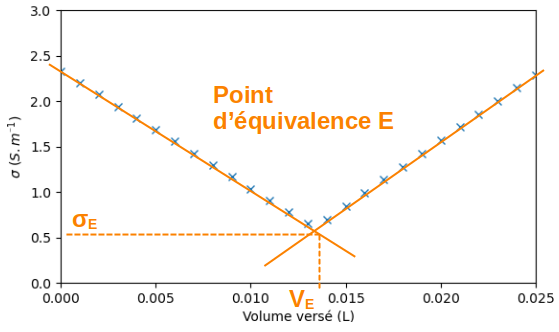
\includegraphics[width=\linewidth]{Ressources/TSPE_C3_Fig10.png}
	\end{center}
	\end{minipage}
\end{figure}
\textbf{Solutions disponibles}
\begin{itemize}
	\item solution de Destop\textsuperscript{\textregistered} diluée 100 fois ($S_1$)
	\item solution d'acide chlorhydrique à \SI{3,00E-2}{\mole\per\liter}
\end{itemize}

\textbf{Données :}
\begin{itemize}
	\item Masse molaire de la soude : $M(\ce{NaOH})$ = \SI{40}{\gram\per\mole}
	\item Conductivités molaires ioniques à 25°C :
    \begin{itemize}
        \item $\lambda (\ce{Na+})$ = \SI{5,0}{\milli\siemens\meter\squared\per\mole} ;
        \item $\lambda (\ce{HO-})$ = \SI{20,0}{\milli\siemens\meter\squared\per\mole} ;
        \item $\lambda (\ce{Cl-})$ = \SI{7,6}{\milli\siemens\meter\squared\per\mole} ;
        \item $\lambda (\ce{H3O+})$ = \SI{35,0}{\milli\siemens\meter\squared\per\mole}
    \end{itemize}
\end{itemize}

\subsection{Analyser et Raisonner}
La solution commerciale de Destop\textsuperscript{\textregistered} est notée $S_0$. Cette solution étant trop concentrée, il faut la diluer cent fois. Le technicien de laboratoire a préparé 1 litre d'une solution de Destop\textsuperscript{\textregistered} diluée 100 fois et notée $S_1$.
\begin{enumerate}
	\item Indiquer quel matériel a été nécessaire pour réaliser cette solution
	\item Justifier qu'il est possible de réaliser un suivi conductimétrique du dosage
	\item Proposer un protocole expérimental permettant d'effectuer le dosage de la solution de Destop\textsuperscript{\textregistered} dilué. Faire un schéma légendé du montage réalisé.\\
	\begin{center}	\textbf{Appel N° 1} \end{center}
\end{enumerate}

\subsection{Réaliser}
Pour suivre un titrage par conductimétrie, il est nécessaire de respecter certaines contraintes opératoires. En particulier :
\begin{itemize}
	\item Il faut étalonner le conductimètre (voir fiche matériel)
	\item La solution titrée doit être additionnée d'un grand volume d'eau pour pouvoir négliger les effets sur  la conductivité de la dilution liée à l'ajout de solution titrante. Il faudra donc dans un bécher de \SI{400}{mL}, verser environ \SI{200}{mL} d'eau distillée, puis introduire précisément $V_1$ = \SI{10,0}{mL} de la solution $S_1$.
	\item Le titrage s'effectue sous agitation modérée.
\end{itemize}
\begin{enumerate}[resume]
	\item Mettre en œuvre le protocole expérimental proposé précédemment en respectant les indications opératoires ci-dessus
	\item Déterminer le volume à l'équivalence en faisant apparaître les constructions graphiques nécessaires sur la courbe
	\item Déterminer alors la concentration $c_1$ de la solution $S_1$ dosée
	\item En déduire la concentration $c_0$ de la solution commerciale de déboucheur
	\begin{center}	\textbf{Appel N° 2} \end{center}
\end{enumerate}

\subsection{Valider}
Si l'écart entre le résultat expérimental $c_0$ et la valeur annoncée par le fabricant $c_{0, fabricant}$ est inférieur ou égal à deux incertitudes-types, il est possible de considérer que le résultat de la mesure est correct.
 \begin{enumerate}[resume]
	\item Déterminer la concentration en quantité de matière $c_{0, fabricant}$ annoncée par le fabricant
	\item On estime l'incertitude-type $u(A)$ = \SI{0,001}{\mole\per\liter}. Estimer les incertitude-type $u(V_{A,E})$ et $u(V_1)$, puis calculer l'incertitude-type $u(c_0)$ à partir de la relation :
	$$\dfrac{u(c_0)}{c_0} = \sqrt{\left(\frac{u(c_A)}{c_A}\right)^2+\left(\frac{u(V_{A,E})}{V_{A,E}}\right)^2+\left(\frac{u(V_1)}{V_1}\right)^2}$$
	\item Calculer l'écart entre la valeur expérimentale et la valeur annoncée puis conclure
	\begin{center}	\textbf{Appel N° 3} \end{center}
\end{enumerate}
\section*{Comprendre la courbe de titrage}
\begin{enumerate}
	\setcounter{enumi}{10}
	\item Dresser un tableau indiquant : les différentes espèces en présence lors du titrage et l'évolution de la quantité de matière de chacune d'elles avant et après l'équivalence
	\item Rappeler l'expression de la conductivité
	\item À l'aide du tableau précédent et des données, expliquer qualitativement l'allure de la courbe obtenue lors du titrage
\end{enumerate}
\end{document}